\chapter{Machine Learning}

Il machine learning è essenziale per la classificazione dei segnali nelle interfacce uomo-macchina.

\section{Apprendimento Supervisionato e Non}
Nel contesto delle interfacce cervello-macchina, è fondamentale saper ricondurre un insieme di campioni fisiologici ad uno stato o ad un comando preciso (e.g. muovi a destra, stato di relax).
Nel corso si predilige l'approccio \textbf{Supervisionato}, provvisto cioè di \textit{label} (etichette) per ogni dato di input. Il dataset viene classicamente diviso in set di \textit{Training} (per addestrare il modello) e \textit{Testing} (per validare la generalizzazione), facendo attenzione ad evitare i fenomeni di \textit{Overfitting} (il modello impara a memoria i dati di addestramento) e \textit{Underfitting} (il modello non riesce a cogliere le relazioni dei dati).

\subsection{Validazione e Sbilanciamento}
La semplice suddivisione in Train e Test (Holdout) può generare distorsioni dovute alla casualità dello split. Si adopera pertanto la \textbf{K-fold Cross Validation}: il dataset viene diviso in $K$ partizioni (fold); iterativamente, $K-1$ fold addestrano il modello e il rimanente funge da test test, ripetendo $K$ volte. Le metriche finali sono la media delle singole iterazioni.
La validazione deve anche affrontare il problema dello \textbf{sbilanciamento delle classi} (es. molti stati di "relax", pochi di "allarme"). Tecniche comuni includono:
\begin{itemize}
    \item \textbf{Oversampling:} Replicare campioni della classe minoritaria.
    \item \textbf{Undersampling:} Ridurre i campioni della classe maggioritaria.
    \item \textbf{SMOTE:} Creare nuovi campioni sintetici interpolando la classe minoritaria.
\end{itemize}

\section{Algoritmi Principali}
Il corso affronta diversi approcci algoritmici classici per affrontare il task di classificazione, ripresi anche dal punto di vista matematico:
\begin{itemize}
    \item \textbf{Decision Trees (Alberi Decisionali e CART):} Modello predittivo che divide lo spazio delle feature con regole di split. Ad ogni nodo, la miglior split viene scelta minimizzando l'impurità. Le formule di impurità principali sono:
    \begin{itemize}
        \item \textbf{Entropia:} $H(S) = - \sum_{i} p_i \log_2(p_i)$
        \item \textbf{Indice di Gini:} $I_G(S) = 1 - \sum_{i} p_i^2$
    \end{itemize}
    Per prevenire un grave overfitting, i criteri di arresto (stopping criteria) includono: massima profondità dell'albero, minimo numero di campioni per formare una foglia, ed eventuale \textit{pruning} (potatura) ex-post.

    \vspace{0.5cm}
    \begin{figure}[h!]
        \centering
        \begin{tikzpicture} [
            node distance=1.5cm and 2cm,
            mynode/.style={draw, rectangle, rounded corners, fill=blue!10, text width=2.5cm, align=center},
            leafnode/.style={draw, rectangle, rounded corners, fill=green!20, text width=2cm, align=center}
        ]
            \node[mynode] (root) {Feature $X_1 > 5$ ? \\ \small Gini: 0.50};
            \node[mynode, below left=of root] (left) {Feature $X_2 < 2$ ? \\ \small Gini: 0.32};
            \node[leafnode, below right=of root] (right) {Classe A \\ \small Gini: 0.00};
            \node[leafnode, below left=of left] (ll) {Classe B \\ \small Gini: 0.00};
            \node[leafnode, below right=of left] (lr) {Classe A \\ \small Gini: 0.15};

            \draw[->, thick] (root) -- node[above left] {Sì} (left);
            \draw[->, thick] (root) -- node[above right] {No} (right);
            \draw[->, thick] (left) -- node[above left] {Sì} (ll);
            \draw[->, thick] (left) -- node[above right] {No} (lr);
        \end{tikzpicture}
        \caption{Esempio di un piccolo Albero Decisionale basato sulla riduzione dell'impurità (Gini).}
    \end{figure}
    \vspace{0.5cm}

    \item \textbf{Random Forest:} Espande il concetto del Decision Tree tramite l'approccio \textbf{Ensemble Learning}. Combina numerosi alberi addestrati su varianti randomiche del dataset (\textbf{Bagging} o Bootstrap Aggregating) estraendo le feature in modo casuale ad ogni split (\textbf{Feature Randomness}). Il risultato finale si ottiene per \textit{Majority Voting}, assicurando eccezionale robustezza e minor overfitting.

    \item \textbf{k-Nearest Neighbors (kNN):} Algoritmo pigro (\textit{lazy learner}) che classifica un nuovo punto analizzando la classe maggioritaria espressa dai suoi $k$ vicini più prossimi (usando distanze come l'Euclidea). Lo spazio può essere rappresentato da \textbf{Diagrammi di Voronoi}.
    \begin{itemize}
        \item \textbf{Effetto di K:} Un $K$ molto piccolo porta a modelli ipersensibili (\emph{Overfitting}, confini rumorosi); un $K$ troppo grande appiattisce il giudizio (\emph{Underfitting}).
        \item \textbf{Normalizzazione:} Cruciale affinché nessuna feature domini il calcolo della distanza a causa della sua scala. Si usano tecniche come Min-Max scaling o Z-score (\textit{Standardization}).
    \end{itemize}

    \item \textbf{Support Vector Machines (SVM):} Modello ampiamente usato nel dominio biomedico per via della capacità di generalizzare in modo robusto in alti spazi dimensionali. Esegue la ricerca dell'iperpiano di separazione che massimizza il margine di distanza dai campioni.
    Matematicamente l'iperpiano è definito da:
    \begin{equation}
        w \cdot x + b = 0
    \end{equation}
    Il margine separatore tra le classi corrisponde a $\frac{2}{||w||}$. Per massimizzarlo si ricorre all'ottimizzazione convessa.
    Nella realtà le classi non sono mai perfettamente separabili. Si introducono le \textbf{Variabili Slack} ($\xi$) per tollerare misclassificazioni, regolate dal parametro $C$ (\textit{Soft Margin}): un $C$ grande impone confini severi, abbassando gli errori sui dati di training ma alzando il rischio di overfitting. Un $C$ piccolo permette un margine più ampio e tollera più errori, migliorando la generalizzazione.
    Infine, si sfrutta il \textbf{Kernel Trick} (es. Polinomiale, RBF - Radial Basis Function) per mappare implicitamente e a basso costo computazionale le feature in uno spazio dimensionale superiore per superare la non-linearità.

    \begin{figure}[h!]
        \centering
        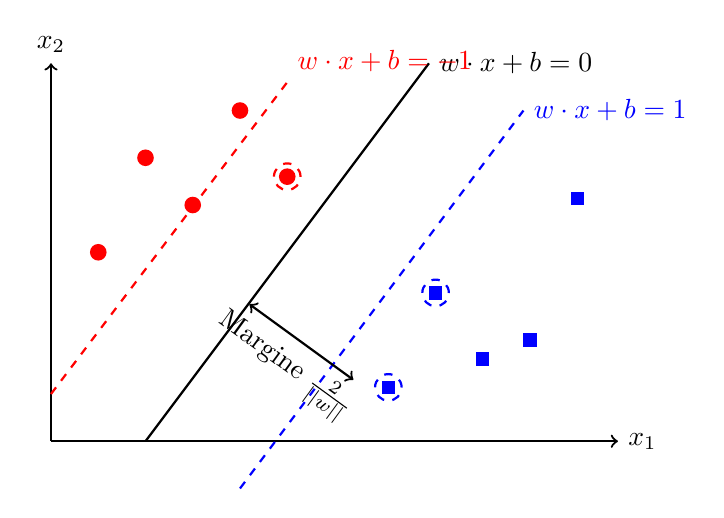
\begin{tikzpicture}[scale=1.2]
            % Asse coordinate
            \draw[->,thick] (0,0) -- (6,0) node[right] {$x_1$};
            \draw[->,thick] (0,0) -- (0,4) node[above] {$x_2$};

            % Punti Classe - (rossi, cerchi)
            \foreach \x/\y in {1/3, 1.5/2.5, 2/3.5, 0.5/2, 2.5/2.8}
                \fill[red] (\x,\y) circle (2.5pt);

            % Punti Classe + (blu, quadrati)
            \foreach \x/\y in {3.5/0.5, 4/1.5, 5/1, 5.5/2.5, 4.5/0.8}
                \fill[blue] (\x,\y) rectangle ++(4pt,4pt);

            % Support Vectors
            \draw[red, thick, dashed] (2.5,2.8) circle (4pt); % SV rosso
            \draw[blue, thick, dashed] (4+0.07,1.5+0.07) circle (4pt); % SV blu
            \draw[blue, thick, dashed] (3.5+0.07,0.5+0.07) circle (4pt); % SV blu 2

            % Iperpiani
            \draw[thick, black] (1,0) -- (4,4) node[right, black] {$w \cdot x + b = 0$};
            \draw[thick, red, dashed] (0,0.5) -- (2.5,3.8) node[above right] {$w \cdot x + b = -1$};
            \draw[thick, blue, dashed] (2,-0.5) -- (5,3.5) node[right] {$w \cdot x + b = 1$};

            % Margine
            \draw[<->, thick] (2.1, 1.45) -- (3.2, 0.65) node[midway, sloped, below] {Margine $\frac{2}{||w||}$};
        \end{tikzpicture}
        \caption{Rappresentazione concettuale di una SVM lineare bidimensionale. Sono evidenziati i vettori di supporto e le equazioni degli iperpiani corrispondenti al margine massimo.}
    \end{figure}

    \item \textbf{Logistic Regression (Regressione Logistica):} Algoritmo parametrico che restituisce, tramite la \textbf{funzione Sigmoide} $\sigma(z) = \frac{1}{1 + e^{-z}}$, la probabilità di appartenenza a una classe (da 0 a 1). La funzione di costo (\textbf{Loss}) è la Log-Loss (o Cross-Entropy), la quale è matematicamente garantita essere \textbf{convessa}: questo assicura che l'algoritmo di ottimizzazione tramite iterazioni di \textbf{Discesa del Gradiente} convergerà sempre a un unico minimo globale ottimale, senza impantanarsi in minimi locali.

    \vspace{0.5cm}
    \begin{figure}[h!]
        \centering
        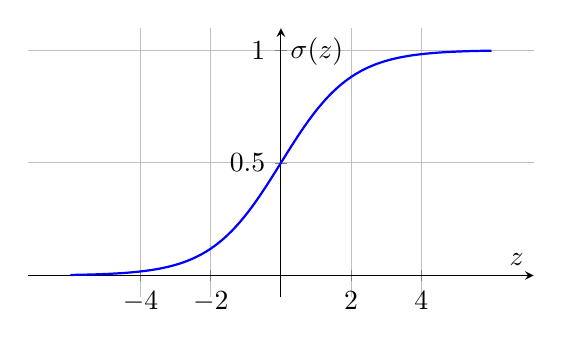
\begin{tikzpicture}
            \begin{axis}[
                width=8cm, height=5cm,
                domain=-6:6, samples=100,
                axis lines=middle,
                xtick={-4,-2,0,2,4},
                ytick={0, 0.5, 1},
                xlabel=$z$, ylabel=$\sigma(z)$,
                enlargelimits=true,
                grid=both
            ]
            \addplot[blue, thick] {1 / (1 + exp(-x))};
            \end{axis}
        \end{tikzpicture}
        \caption{Funzione Sigmoide utilizzata nella Logistic Regression per mappare un valore reale $z$ in una probabilità $(0, 1)$.}
    \end{figure}
    \vspace{0.5cm}
\end{itemize}

\section{Metriche di Valutazione}
Per quantificare l'efficienza degli algoritmi di classificazione, ci si affida sovente all'uso della \textbf{Matrice di Confusione}, che espone i True Positive (TP), True Negative (TN), False Positive (FP) e False Negative (FN). Da questa matrice si ricavano formule essenziali:
\begin{itemize}
    \item \textbf{Accuracy (Accuratezza):} Percentuale di predizioni corrette totali, calcolata come $\frac{TP + TN}{TP + TN + FP + FN}$. Può essere ingannevole se il dataset è sbilanciato.
    \item \textbf{Precision (Precisione):} Rapporto dei positivi previsti in modo corretto sui positivi totali predetti $\frac{TP}{TP + FP}$.
    \item \textbf{Recall (Sensibilità):} Rapporto dei positivi individuati sul totale dei positivi reali $\frac{TP}{TP + FN}$. Utile in ambito medico per minimizzare i falsi negativi.
    \item \textbf{F1-Score:} Media armonica pesata di Precision e Recall.
\end{itemize}

\section{Estrazione di Features (Feature Extraction)}
Prima di alimentare i modelli (in particolar modo nel caso SVM, ma per tutti limitatamente alle performance), occorre fornire al modello solo dati salienti per evitare il fenomeno della \textit{Curse of Dimensionality} (Maledizione della dimensionalità). Per i segnali fisici si estraggono perciò parametri \textbf{temporali} (es. deviazione standard, media e andamento del battito ECG) e/o \textbf{frequenziali} (come la \textit{Power Spectral Density} nei casi dell'EEG ritrati ritmati come Alpha, Beta o Theta \textit{Waves}).
